\documentclass[12pt,a4paper]{ctexart}

\usepackage[a4paper,margin=2.5cm]{geometry}
\usepackage{array}
\usepackage{booktabs}
\usepackage{caption}
\usepackage{graphicx}
\usepackage{hyperref}
\usepackage{setspace}
\usepackage{tabularx}
\usepackage{titlesec}

\hypersetup{hidelinks}
\setstretch{1.35}
\emergencystretch=2em
\setcounter{tocdepth}{3}
\setcounter{secnumdepth}{3}

\titleformat{\section}{\heiti\zihao{-3}}{\thesection}{1em}{}
\titleformat{\subsection}{\heiti\zihao{4}}{\thesubsection}{1em}{}
\titleformat{\subsubsection}{\heiti\zihao{-4}}{\thesubsubsection}{1em}{}

\captionsetup[table]{skip=6pt}

\begin{document}

\begin{center}
    {\zihao{3}\heiti 中期报告工作进展：力学系统自动形式化流水线部分}
\end{center}

\section{力学系统自动形式化流水线工作进展}

\subsection{研究目标与总体设计}

本课题中的力学系统自动形式化流水线，旨在将自然语言题目逐步转化为可由 Lean 形式化系统检查的命题与证明对象，并在此过程中尽量保持题意、目标量、约束条件和物理规律的一致性。与直接让模型一次性输出最终形式化结果的做法不同，本课题采用分阶段流水线设计，其核心考虑在于：力学题目的自动形式化并非单一生成任务，而是题目理解、知识调用、命题构造、编译检查、语义筛选和证明验证共同构成的复合过程。如果缺乏分阶段约束，系统虽然可能生成表面上类似 Lean 代码的文本，却难以保证其在真实形式化环境中的可执行性与可验证性。

基于这一认识，项目在中期阶段形成了一条较为完整的自动形式化主流程。该流程不是以单个模型调用为中心，而是围绕“生成之后必须经过真实验证”这一原则组织的。系统先对题目进行结构化理解，再生成多个候选命题，随后以真实 Lean 编译结果和语义一致性分析作为筛选标准，最后对选中候选进行证明生成与证明校验，并将整个过程写入结构化产物和导出工作区。该设计使流水线不仅能够给出最终结果，而且能够说明中间阶段的状态变化与失败原因，从而满足研究型系统对可追溯性和可分析性的要求。

\subsection{流水线总体结构}

当前实现的力学系统自动形式化流水线可概括为“题目输入、结构化理解、知识注入、候选生成、编译验证、语义排序、证明验证、结果归档”八个环节。其总体结构如图~\ref{fig:pipeline-overview} 所示。

\begin{figure}[htbp]
    \centering
    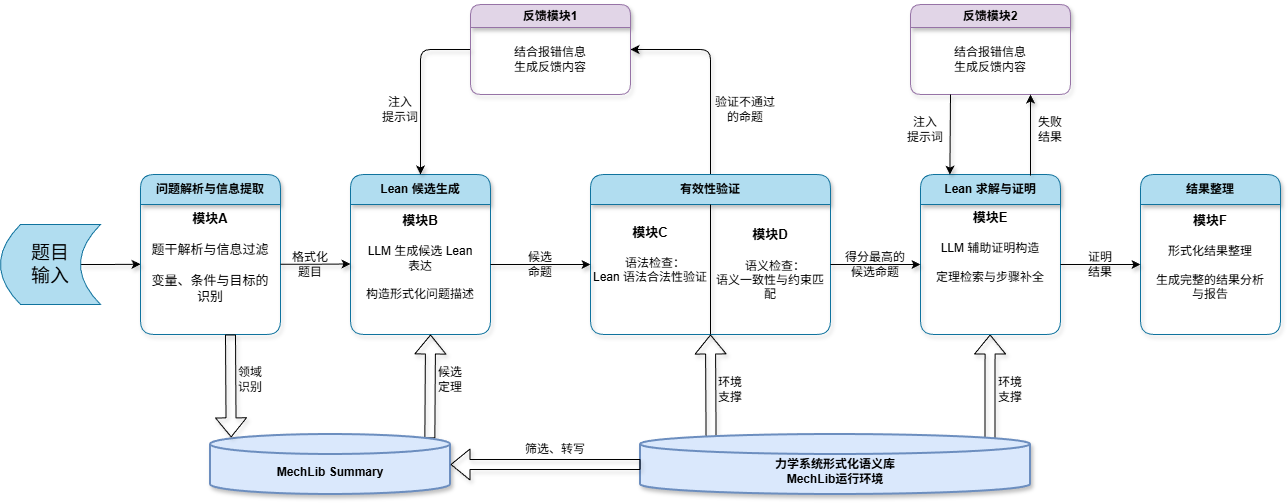
\includegraphics[width=0.95\textwidth]{pipeline.png}
    \caption{力学系统自动形式化流水线示意图}
    \label{fig:pipeline-overview}
\end{figure}

从系统结构上看，该流水线具有两个显著特征。第一，它采用串联式分阶段组织，而不是将全部任务压缩为一次端到端生成；第二，它在生成阶段与验证阶段之间设置了真实的外部判据，即 Lean 编译器与 Lean 证明检查器。前者用于判断候选命题是否在语法、类型和库依赖层面成立，后者则用于判断命题是否能够被证明或修复到可证明状态。正因为存在这两层真实约束，流水线输出才能被视为具有研究意义的“形式化结果”，而不是仅仅停留于自然语言模型生成的文本片段。

\subsection{各阶段功能与当前实现}

\subsubsection{题目输入与结构化理解}

流水线的起点是题目输入。当前系统已支持多种数据来源，包括标准基准数据集、本地归档题目以及自建专题测试集。进入流水线后，系统首先对题面进行清洗、标准化与统一封装，并构造题目的结构化表示。该结构化表示的核心任务，是将题目中的物理对象、已知条件、求解目标、单位信息和规律线索抽取为统一的数据结构，从而为后续模块提供稳定输入。

这一阶段的重要性在于，它将原本高度自由、表述差异很大的自然语言题目转换为后续模块可共享的中间语义对象。由此，候选命题生成模块不必直接面对原始题面中的全部噪声，而可以基于结构化结果开展更稳定的命题构造。就研究目标而言，这一部分承担的是“题目语义接口层”的作用；就流水线实现而言，它决定了系统后续所有阶段的输入质量。

\subsubsection{知识注入与候选命题生成}

在结构化理解之后，流水线会根据题目主题和规律线索调用知识检索模块，为后续命题生成提供相关形式化上下文。随后，候选命题生成阶段在题干信息、结构化表示和知识上下文的共同约束下，构造多个 Lean 命题候选。这些候选并不是简单的同义改写，而是试图从不同建模角度给出可能的形式化表达，以提高后续阶段找到正确命题的概率。

中期阶段的重要进展之一，是命题生成模块已经不再停留在“输出若干 theorem 字符串”的粗糙状态，而是逐步转向“带依据的候选构造”。当前系统已经能够为候选记录其支持事实、来源类型和潜在库符号，并在局部层面识别缺少依据的声明。这一改造使候选命题不再只是无来源的形式表达，而开始具备“来自题干条件或理论库”的可追溯性。这对于后续语义排序尤其重要，因为它使系统不仅能比较“哪个候选更像题意”，还可以进一步比较“哪个候选更有形式化依据”。

\subsubsection{编译检查与语义排序}

候选命题生成完成后，系统不会直接进入证明，而是先通过 Lean 编译阶段对每个候选进行检查。该阶段调用真实的 Lean 环境，对候选命题逐一进行语法、类型、头文件依赖和库接口层面的编译验证。只有通过编译检查的候选，才有资格进入后续的语义排序阶段。

在编译检查之后，流水线进一步通过语义排序模块判断候选命题与原题之间是否真正一致。这一阶段并不只比较表面文字相似性，而是结合目标量、已知量、物理规律、约束条件和反向解释结果，对候选进行更细粒度的语义判别。中期阶段的一个重要进展，是系统已经能够区分“完全一致”“形式不同但语义等价”“特例化”“弱化”和“语义偏离”等多种关系，从而避免将表面形式差异误判为完全错误，也避免让过于弱化或平凡化的命题轻易通过筛选。

\subsubsection{证明生成、修复与最终验证}

对于通过语义排序的候选，流水线会进入证明阶段。该阶段的目标并不是单纯生成一段看似合理的 tactic，而是构造能够在真实 Lean 环境中通过验证的证明对象。当前系统中，证明阶段已经从早期的单步生成演化为更细的分阶段策略：先围绕候选命题生成证明计划，再根据计划生成具体 Lean 证明；若初次证明失败，则结合错误信息进行有限轮次的修复。

这一阶段的意义在于，它使流水线不再停留在“命题对了即可”的层面，而是进一步追问“该命题是否能够在形式系统中被证明”。从中期实验结果来看，证明阶段已经成为当前系统最主要的性能瓶颈之一。这也意味着前面题目理解、命题生成、编译检查和语义筛选等环节已经取得一定效果，后续研究的重点需要更明确地转向证明规划、证明修复以及定理复用能力的提升。

\subsubsection{反馈闭环与结果归档}

为了避免一次性失败直接终止整道题，当前流水线在命题生成、编译检查和语义排序之间已经形成单轮反馈闭环。当所有候选在编译阶段失败，或虽可编译但未能通过语义排序时，系统会将错误摘要结构化后反馈给候选生成模块，用于进行一次针对性的修订。这种设计的意义在于，它使流水线从静态单次生成转向了有限度的动态修正，提高了在复杂题目上的容错能力。

在整次运行完成后，系统会自动输出指标汇总、阶段日志、样本级结果文件、分析报告和可独立打开的 Lean 工作区。由此，实验不再依赖人工记录或零散日志，而能够被完整归档和复查。对于研究工作而言，这一归档能力具有重要意义，因为它使每一次实验都具备可重现、可对比和可追溯的基本条件。

以最近一次在 $101$ 道标准力学题集上的全量主流程运行为例，系统在各阶段的样本级成功数量已经可以被稳定统计：题目结构化理解成功 $98/101$，候选命题生成成功 $97/101$，编译检查成功 $78/101$，语义一致性筛选成功 $22/101$，证明验证成功 $15/101$，最终端到端完成形式化验证的题目为 $15/101$。这一结果表明，当前流水线前半段已经能够较稳定地完成题目理解与候选生成，而主要性能损失集中在编译之后的语义筛选与证明阶段。

\subsection{已完成的关键工程工作}

\subsubsection{形成了稳定的多源输入与统一配置机制}

中期阶段已经完成数据输入、模型接口、Lean 环境、知识检索、输出目录和并发参数的统一配置管理。这意味着流水线不再依赖手工修改脚本和临时路径，而是能够通过结构化配置文件稳定控制实验行为。该机制对后续 benchmark 运行、专题测试和消融实验具有直接支撑作用。

\subsubsection{形成了真实形式化环境下的执行闭环}

当前流水线的一个关键特点，是其每一轮候选命题和最终证明都要经过真实 Lean 环境的检查。这一设计使实验结果具备明确的外部判据，从而避免了“模型输出看似合理但实际不可执行”的问题。对中期阶段而言，这种执行闭环已经是最重要的工程性成果之一，因为它将整个研究对象从“自然语言转代码”提升为“自然语言转可验证形式对象”。

\subsubsection{形成了题目级并发与进度监控机制}

考虑到真实 API 调用与 Lean 检查的运行成本较高，系统在中期阶段已经引入题目级并发机制，并能够在长批量实验中实时显示完成进度。这一改造并未改变单题内部的处理顺序，而是通过题目级调度提高总体实验吞吐。配合完整的归档机制，该设计使系统能够支撑一百题量级的全量测试，并满足中期阶段对多轮实验对比的现实需求。

\subsubsection{形成了结构化诊断与结果分析能力}

中期阶段还完成了对失败类型、子错误类型和阶段性错误摘要的结构化记录。系统目前已经能够区分语义偏离、证明搜索失败、命题形状错误、编译超时等不同失败模式，并将其写入样本级结果和分析报告。由此，流水线的价值不再仅仅体现在“能否成功”，还体现在“能否说明失败发生在何处、为何发生以及是否可修复”。这一点对于研究型项目尤为重要，因为后续所有改进都必须建立在可靠的错误归因基础之上。

\subsection{阶段性认识}

\subsubsection{流水线主体结构已经形成，研究重点正在向后半段转移}

综合当前代码实现与实验结果，可以确认力学系统自动形式化流水线的主体结构已经建成。题目输入、结构化理解、候选生成、编译检查、语义排序、证明验证和结果归档等环节均已具备稳定实现，并能够支撑真实数据集上的完整运行。这说明课题在中期阶段已经完成了从“概念性方案”向“可复现实验系统”的关键转换。

与此同时，流水线各环节的重要性已经发生变化。早期阶段的主要困难在于能否把题目成功转写为可编译的 Lean 命题；而从当前实验看，系统的主要瓶颈已经逐渐转移到语义筛选和证明阶段，特别是复杂题目下的证明规划与修复能力不足。这一变化说明前半段自动形式化工作已取得实质进展，也为下一阶段明确研究重点提供了依据。

\subsubsection{当前流水线已具备研究价值，但仍需进一步提升知识复用与证明能力}

当前流水线已经能够在真实 Lean 环境中完成较大规模实验，并形成系统性的样本级分析结果，因此从研究方法上看，它已经具备了较明确的实验平台价值。然而，中期阶段的结果同样表明，系统虽然已经实现知识检索注入和结构化候选生成，但知识上下文尚未稳定转化为最终命题与证明中的显式定理复用；同时，证明阶段仍是制约端到端成功率的主要因素。

因此，流水线后续改进的重点不应再停留在单纯增加候选数量或继续堆叠提示信息，而应更明确地转向两个方向：一是提升候选命题的依据化程度，使正确且有来源支撑的候选能够在排序中胜出；二是强化证明计划与库定理调用能力，使系统从“能够生成可编译命题”进一步提升为“能够稳定生成可验证证明”。这两点将直接决定流水线能否从中期基线进一步发展为具有较强形式化推理能力的研究系统。

\subsection{小结}

总体而言，中期阶段在力学系统自动形式化流水线方向已经取得了较为扎实的阶段成果。当前系统已经形成从题目输入到 Lean 导出工作区的完整主流程，具备多源数据接入、知识注入、候选生成、编译检查、语义排序、证明验证、反馈修订与结果归档等关键能力，并能够在真实 API 和真实 Lean 环境下完成中等规模以上实验。这一进展说明课题已经完成了自动形式化研究中最关键的工程基线搭建工作。

同时，中期结果也清晰地揭示了当前流水线的真实边界：前半段自动形式化链路已经基本打通，但后半段证明与知识复用能力仍需重点加强。因此，关于流水线部分的中期结论可以概括为：\emph{项目已经建立起可复现、可验证、可诊断的力学自动形式化主流程，为后续围绕定理复用、证明规划和复杂题型处理的进一步研究奠定了稳定基础。}

\end{document}
